% WORKAROUND (an update of the geometry package broke beamer...)
\makeatletter\let\ifGm@compatii\relax\makeatother
% end of WORKAROUND


\documentclass{beamer}
% \usetheme[uttitlepage=false]{ut}
\usetheme[euler=false,titlepage=B]{ut}
%\usetheme[titlepage=C,debug]{ut}


\graphicspath{{/home/andrea/Pictures/ImagesDutchPres/}}

\title{Presentatie van de Nederland cursus}
% \subtitle[Short subtitle]{I am not using any subtitles}
\author[A.~Brugnoli]{Andrea Brugnoli} %  
\institute[UT]{Department of Robotics and Mechatronics,\\ University of Twente}
%\date[29-04-2021]{April 29, 2021}
\footlinetext{[A.~Brugnoli]}

% \titlegraphic{\includegraphics[height=1cm]{titlegraphic}}

% \utbeamerset{tpboxbx=10}

\begin{document}
	
	\maketitle
	
	\begin{frame}{Wie ben ik?}
		Het is jammer dat we elkaar niet persoonlijk leren kennen. Met deze presentatie zal ik proberen mijzelf voor te stellen en de levenservaringen die mij naar Nederland hebben gebracht, te delen. 
	\end{frame}

	
	\begin{frame}{Mijn woonplaats}
		Ik ben geboren in Verona. Verona ligt in het noorden van Italië, ten westen van Venetië. Het is gebouwd rond de rivier de Adige.
	\begin{figure}
		\centering
		\includegraphics[width=1\textwidth]{verona.jpg}
		\caption{Historisch centrum van Verona}
	\end{figure}
	\end{frame}

	\begin{frame}{De Arena}
		Het historische centrum is beschermd door de UNESCO en bevat een goed bewaarde Romeinse arena en vele middeleeuwse kerken.
		\begin{figure}
			\centering
			\includegraphics[width=1\textwidth]{arena.jpg}
			\caption{Arena van Verona}
		\end{figure}
	\end{frame}	

	\begin{frame}{Valpolicella}
		Mijn familie woont op het westelijke platteland, in Valpolicella.
		\begin{figure}
			\centering
			\includegraphics[width=1\textwidth]{valpolicella.jpg}
			\caption{De Valpolicella wijnbouwgebied}
		\end{figure}
	\end{frame}	

	\begin{frame}{Gardameer}
		Vlakbij Valpolicella, ligt het grootste Italiaanse meer, het Gardameer.
	\begin{figure}
		\centering
		\includegraphics[width=.8\textwidth]{garda.jpg}
		\caption{Punta San Vigilio}
	\end{figure}
	\end{frame}

	\begin{frame}{Milan}
		Na de middelbare school ben ik voor mijn studie naar Milaan gegaan.
		\begin{figure}
			\centering
			\includegraphics[width=.8\textwidth]{milano.jpg}
		\end{figure}
	\end{frame}

	\begin{frame}{Toulouse}
		Tijdens mijn masterstudie had ik de mogelijkheid om naar Toulouse te gaan.
		\begin{figure}
			\centering
			\includegraphics[width=.75\textwidth]{toulouse.jpg}
			\caption{De rivier de Garonna doorkruist het centrum van Toulouse.}
		\end{figure}
	\end{frame}

	\begin{frame}{Canal du midi}
		\begin{figure}
			\centering
			\includegraphics[width=.8\textwidth]{canal-du-midi.jpg}
			\caption{Het is mogelijk om langs het kanaal van Toulouse tot aan de Middellandse Zee te fietsen.}
		\end{figure}
	\end{frame}

	\begin{frame}{Brazil}
		Tijdens mijn PHD heb ik vier maanden in Brazilië doorgebracht. Ik verbleef in São José dos Campos.
		\begin{figure}
			\centering
			\includegraphics[width=.8\textwidth]{sao-jose.jpeg}
			\caption{São José dos Campos}
		\end{figure}
	\end{frame}

	\begin{frame}{Braziliaans carnaval}
		Historisch gezien bestond het carnaval uit groepen die door de lanen van de stad paradeerden en dansten.
		\begin{figure}
			\centering
			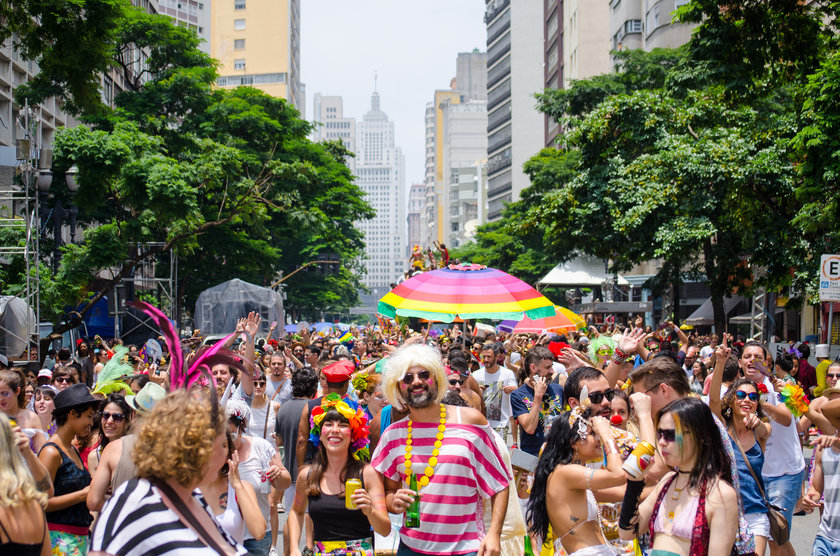
\includegraphics[width=.8\textwidth]{carnaval-sao-paulo.jpg}
			\caption{Een bloco in Sao Paulo}
		\end{figure}
	\end{frame}

\begin{frame}{Natuur in Brazil}
	Brazilië heeft een ecosysteem dat meer aanwezig is in de steden zelf.
	\begin{figure}
		\centering
			\includegraphics[width=0.7\textwidth]{rio-cristo.jpg}
		\caption{Cristo redentor panorama}
	\end{figure}
\end{frame}

\begin{frame}{Natuur in Brazil}
	\begin{figure}
		\centering
		\includegraphics[width=0.8\textwidth]{trinidade.jpg}
		\caption{Trinidade strand}
	\end{figure}
\end{frame}

\begin{frame}{Conclusie}
	Ik doe nu een post-doc in Enschede. Ik hou van de manier van leven hier: de stad is klein maar alle voorzieningen zijn dichtbij. De mensen zijn erg vriendelijk en bereid om te helpen. \\ 
	
	\vspace{1cm}
	Het is nu tijd om de presentatie af te sluiten. Ik heb erg genoten van deze cursus en ik ga waarschijnlijk in september verder. 
\end{frame}

	
\end{document}

